\part{Prerequisites for Machine Learning in ECL}\label{part:prereqs}

\chapter{Introduction}\label{chap:intro}

Machine learning and Artificial Intelligence are growing at a tremendous rate in the technological world, and most software engineers need knowledge on these fields in order to keep up with the industry.

This brings into light about how training a lot of these models on a large amount of data may take a large amount of time and processing power. To solve these issues, distributed computing was introduced.

Distributed computing is a field of computer science that studies systems whose components are located on different networked computers, which communicate and coordinate their actions by passing messages to one another from any system.

In this document, we shall focus on one such open source distributed system, HPCC Systems. HPCC Systems uses it's own declarative programming language for processing data, which is known as Enterprise Control Language or ECL.

This document assumes that the reader has idea about the following concepts of ECL:
\begin{itemize}
    \item Syntax, Operators
    \item Datasets, Records and Datatypes
    \item Aggregate functions
    \item Sort, Iterate, Rollup, Dedup, Join
    \item Output and Export
    \item Project, Transform, Normalize, Denormalize, Distribute
    \item Functions, Modules and Bundles
\end{itemize}

\section{How to use this document}\label{sec:howtouse}

The best way to use this document would be refer to the parts as it is required by the user after reading through Part \ref{part:prereqs}.

This document is used to help the reader understand how to implement ML algorithms in HPCC systems, but it will be much more useful as a quick reference to using the most important ML methods developed in ECL until \today.

For example, if you ever had to understand how to perform linear regression on your dataset, you could just go to the table of contents to click on the specific part of the linear regression section to make your workflow easier and more convenient.

\section{Supervised vs Unsupervised learning - An overview}\label{sec:supe_vs_unsupe}

Supervised and Unsupervised learning differ in the type of data given to them and in the way they learn. Below is a comic of different kind of robots ranting to each other. Do you think you can figure out the type of learning means from it?

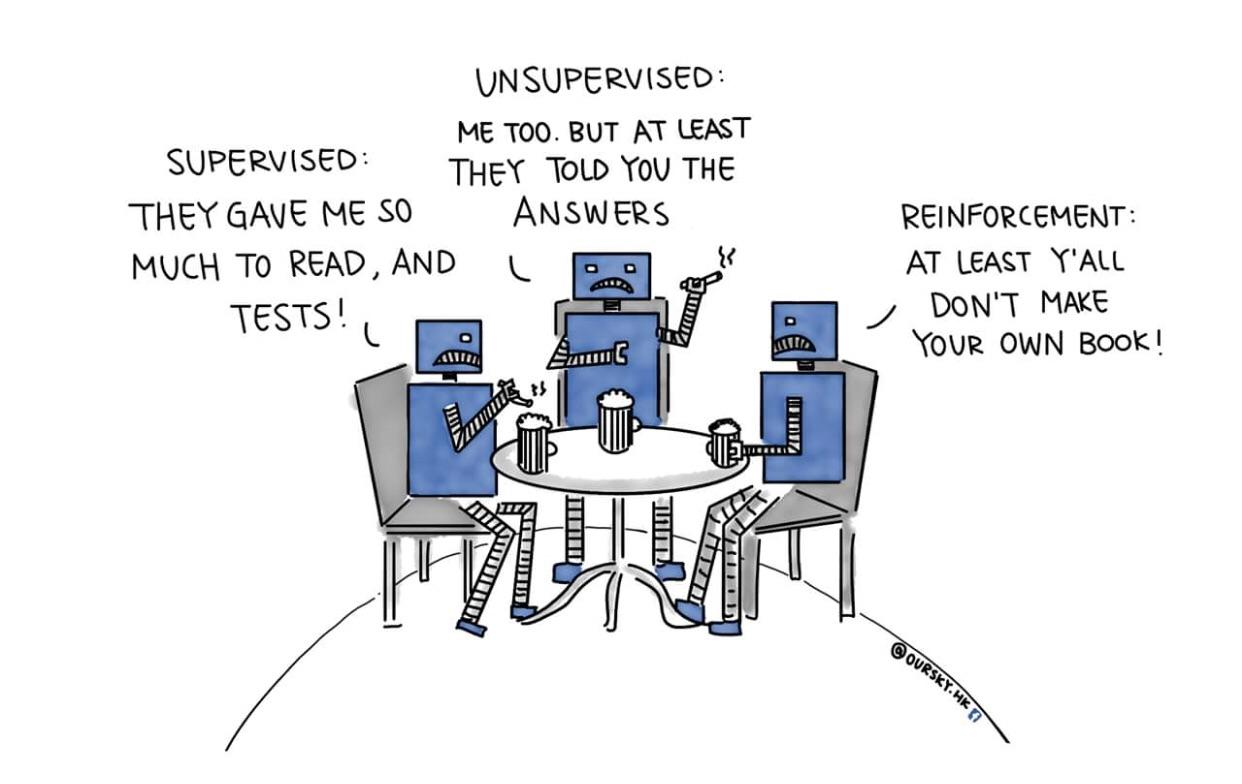
\includegraphics[width=\textwidth]{../media/intro/learningtypes.jpg}

\subsection{Supervised learning}\label{subsec:supe}

When a model trains with data that is well "labelled", and on basis of the given data predicts the output, it is called Supervised learning. It is called so because the training data provided to the model work as the supervisor that teaches the machine to predict correctly. 

Simply explained, the data is like a teacher supervising a student. The teacher must correct the student by showing an example over and over until the student perfectly learns from the examples. The data given to the model acts like the teacher, and is the primary inspiration for the model to predict correctly. 

That being said, it is true that with an incompatible teacher, it might do more worse than good. An teacher specialising in history would be very bad for a student who wants to learn science, and is very interested in it. Just like this, data must be right for the model or it just causes more damage.

Mathematically explained, the aim of supervised learning is to find out the best fitting function $f$ in the equation: \[y=f(x)\] where, $y$ is the predicted output and $x$ is the input variable. 

Supervised learning requires carefully labelled data by a supervisor in order to train the model, and test the accuracy of it to understand and improve the model further.

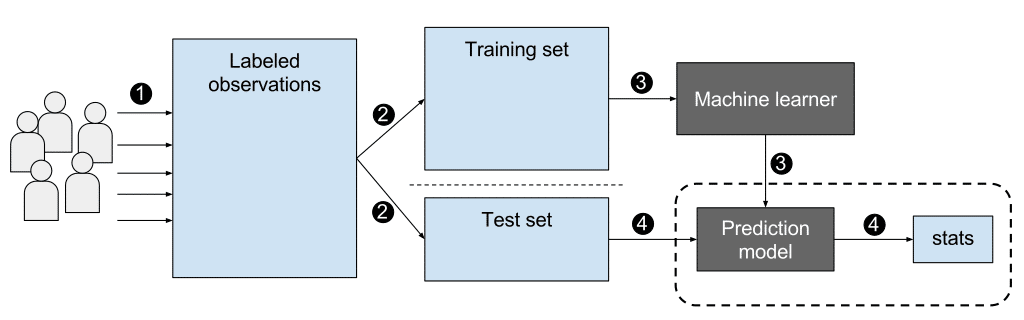
\includegraphics[width=\columnwidth]{../media/intro/Supervised_machine_learning_in_a_nutshell.svg_.png}

The above image explains how supervised learning works in a nutshell. All supervised learning models have the following series of steps that are required to be performed:

\begin{enumerate}
    \item Preparation of labelled data
    \item Pre-processing of data to be compatible with model
    \item Splitting data into train and test sets
    \item Definition of a mathematical model for learning
    \item Train or Fit the model with training set
    \item Test the model with the test set, and calculate accuracy
    \item If accuracy is good enough, use model to predict with real data
\end{enumerate}

That being said, there are many examples of supervised learning models, but the ones available in HPCC Systems developed using ECL or C++ are: 

\begin{itemize}
    \item \nameref{supe:linreg}
    \item \nameref{supe:logreg}
    \item \nameref{supe:svm}
    % \item \nameref{supe:glm}
    \item \nameref{supe:learntrees}
    % \item \nameref{supe:gnn}
\end{itemize}

All the above listed bundles are explained in the following document in Part \ref{part:supe}.

\subsection{Unsupervised learning}\label{subsec:unsupe}

When a model trains with data that is unlabelled, and are allowed to act on the data without supervision, it is called Unsupervised learning. Unlike in supervised learning, the data does not act as a supervisor to the model.

Simply explained, here the data is like homework provided by the teacher to the student. The student must look at the homework, and based on existing knowledge must figure out patterns, and extrapolate answers. Just like this, in unsupervised models, there are no corrections done, but the model must work on the data without supervision in order to learn from the patterns in the data, because the data doesn't have answers provided in it. 

Here as well, it is true that with homework that don't have existing patterns or are beyond the scope of the student will be filled by bizarre answers by the student. Similarly, if a certain dataset is beyond the scope of an unsupervised model, it will provide bizarre results.

Unsupervised learning requires unlabelled data along with a specific model with the perfect parameters to yield the best results. The model fits onto the dataset, and then is tested to check for best results. Then the model is further improved until it works best for the dataset provided.
\\

All unsupervised learning models have the following series of steps that are required to be performed:

\begin{enumerate}
    \item Ponder on the application and the kind of data being used
    \item Choose the model appropriately
    \item Preprocess the data to be compatible with the model
    \item Define the mathematical model that will be used
    \item Split the dataset into train and test sets
    \item Fit the train data to the model
    \item Test the model with the test set, and calculate accuracy
    \item If accuracy is good enough, use model to work with real data
\end{enumerate}

There are many examples of unsupervised learning models, but the ones available in HPCC Systems developed using ECL or C++ are:

\begin{itemize}
    \item \nameref{unsupe:kmeans}
    \item \nameref{unsupe:dbscan}
\end{itemize}

All the above listed bundles are explained in the following document in Part \ref{part:unsupe}

\chapter{The Core and Building Blocks of ML}\label{chap:coreml}

All these Machine Learning algorithms have a lot of mathematics with topics spanning over Linear Algebra, Calculus, Statistics, Probability, Geometry and Decision theory as well. 

Most of the algorithms are a combination of multiple mathematical operations/functions used together in all steps of performing machine learning. 

The most commonly used ones need to be written in the most optimised manner for the ease of the data scientist/programmer so they can focus on the ML algorithm or task at hand instead of needing to gain a deep understanding of how each mathematical operation and function work to implement them, and then putting them together for the ML algorithm.

This is where the bundles \nameref{sec:mlcore} and \nameref{sec:pbblas} come in. These bundles contain the most essential mathematical functions that are used in the ML algorithms to give a simple interface for the user of HPCC to work with the models and datasets conveniently.

\section{ML Core}\label{sec:mlcore}

ML Core simply abbreviates to "Machine Learning Core", and it defines the required functions that are needed for Data Manipulation, Analysis and Model evaluation. This section will be covering about the installation, usage and the most commonly used functions in ML Core.

\subsection{Installation}

To install this bundle, the user needs to run the following command:

\lstinputlisting[caption=Install ML Core Bundle]{source/ml/mlcore/install.sh}

This will install the latest stable version of ML Core from the official repository.

\subsection{Usage}

Although the bundle is installed, the user still needs to IMPORT the bundle into their ECL code. The required functions need to be imported and used accordingly as per the use case.

An example given below shows the usage of an important macro \textbf{\nameref{mlcore:tofield}}:

\lstinputlisting[caption=ToField Example]{source/ml/mlcore/tofield.ecl}

There's a deep documentation file of ML Core that can be accessed on the HPCC website on the following link: \url{https://cdn.hpccsystems.com/pdf/ml/ML\_Core.pdf}. This documentation has the official declaration of parameters, return types and bundle structure. This can be used for reference and importing from ML Core properly. This document goes with a more example-oriented approach to understand the bundles described.

\subsection{Commonly used functions}

\subsubsection{ToField}\label{mlcore:tofield}

\textit{Converts a record-oriented dataset to a cell-oriented NumericField dataset for use with Machine Learning mechanisms}

\paragraph{Explanation}

By \textbf{Record-oriented dataset}, it really refers to most ECL datasets that really on a specific record. For example, I can have id, name, email id, date of birth be defined as a record like this:

\begin{lstlisting}
exampleRec := RECORD
    INTEGER id;
    STRING name;
    STRING emailid;
    DATE dob;
END;
\end{lstlisting}

The problem with this kind of structure is that specific cells of data cannot be dealt with easily. I would have to ingest record-by-record, which may not be correct for ML operations as a few attributes will not be needed at all.

To solve this issue, certain uniform formats for all ML algorithms in ECL are used by ML Core which are NumericField and DiscreteField. These are defined in Types.ecl module in ML Core bundle. These are \textbf{Cell-oriented} which means that data can be handled as independent cells having values with a certain position defined based on column and rowID. More can be read in the documentation that was talked about above.

\paragraph{Example}

Let's look at an example using ML Core to understand better on how to use it.

\lstinputlisting[caption=ToField Example]{source/ml/mlcore/tofield.ecl}

An example record is defined above which defines the shape of each record in the dataset. A dataset is created from a sprayed CSV file in a specific format. This dataset is converted to a Numeric Field for ML applications.

A question might arise: exampleNF is not even defined. How are we giving it as an argument?

This is where the term "Macros" in ECL come into application. A macro does not return anything but new attributes are created in-line for use in subsequent definitions. ToField is a Macro that defines exampleNF for use in further definitions and it does not need to be defined explicitly.

The above code can be run with any CSV file and record to observe the Numeric Field format and get a better understanding of how it works.

\textbf{Note}: All the arguments after exampleRec in the DATASET function in the above example are specific to a CSV file.

\subsubsection{FromField}\label{mlcore:fromfield}

\textit{Macro to convert a NumericField formatted, cell-based dataset to a Record formatted dataset}

\paragraph{Explanation}

This macro does the exact opposite of ToField. It takes a Numeric Field and converts it into a specific record-oriented dataset. 

It really comes to use to convert the output of regressional models into record-oriented dataset to analyse and read better. 

\paragraph{Example}

Let's look at an example of FromField being used

\lstinputlisting[caption=FromField Example]{source/ml/mlcore/fromfield.ecl}

The above example shows how to convert any Numeric Field into a record-oriented dataset given a record. FromField is a macro so exampleDsOut can be used in subsequent lines as it's defined in-line.

\subsubsection{AppendID}\label{mlcore:appendid}

\textit{Macro takes any structured dataset, and appends a unique 1-based record ID column to it. Values will not be sequential and values will not be dense because of data skew. Gaps will appear when data ends on each node. If dense and sequential values are required, use \nameref{mlcore:appendseqid}.}

\paragraph{Example}

Here's an example of AppendID to show it can be used in ECL

\lstinputlisting[caption=AppendID Example]{source/ml/mlcore/appendid.ecl}

NumericField will had IDs by itself when not mentioned, but it's a good practice to append IDs to the dataset by using the Append ID macros. The second argument mentions what the attribute name of the appended ID will be.

\subsubsection{AppendSeqID}\label{mlcore:appendseqid}

\textit{Macro takes any structured dataset, and appends a unique 1-based record ID column to it. Values will be in data sequence. Note: implemented as a count project, each node processes the data in series instead of parallel. For better cluster performance, use \nameref{mlcore:appendid} as long as dense, sequential ids are not needed.}

\paragraph{Example}

Here's an example of AppendSeqID to show how it can be used in ECL

\lstinputlisting[caption=AppendSeqID Example]{source/ml/mlcore/appendseqid.ecl}

NumericField will had IDs by itself when not mentioned, but it's a good practice to append IDs to the dataset by using the Append ID macros. The second argument mentions what the attribute name of the appended ID will be.

\subsubsection{Discretize}\label{mlcore:discretize}

\textit{This module is used to turn a dataset of NumericFields into a dataset of DiscreteFields. This is not quite as trivial as it seems as there are a number of different ways to make the underlying data discrete; and even within one method there may be different parameters. Further - it is quite probable that different methods are going to be desired for each field.}

\paragraph{Functions}

\begin{enumerate}
    \item \textbf{ByRounding}: Round the values passed in to create a discrete element Scale is applied (by multiplication) first and can be used to bring the data into a desired range.
    \item \textbf{ByBucketing}: Allocates a continuous variable into one of N buckets based upon an equal division of the RANGE of the variable.
    \item \textbf{ByTiling}: Allocate a continuous variable into one of N groups such that each group (tile) contains roughly the same number of entries and that all of the elements of group 2 have a higher value than group 1, etc.
\end{enumerate}

\lstinputlisting[caption=Discretize Example]{source/ml/mlcore/discretize.ecl}

Discretization is important to generate DiscreteField dataset for Classification problems as classifiers rely on DiscreteField and NumericField are incompatible. It's use is shown in the program given in Classification Analysis Example and all classification models in the following document.

\subsubsection{Analysis}\label{mlcore:analysis}

\textit{Analysis is a module in ML Core that has functions defined to analyse the trained models of any kinds to check for it's performance on a certain dataset. }

\paragraph{Classification}\label{analysis:classification}

\textit{This sub-module provides functions for analyzing and assessing the effectiveness of an ML Classification model. It can be used with any ML Bundle that supports classification.}

\subparagraph{Functions}

All of these will be implemented in a further example

\begin{enumerate}
    \item \textbf{ClassStats}: Given a set of expected dependent values, assess the number and percentage of records that were of each class.
    \item \textbf{ConfusionMatrix}: Returns the Confusion Matrix, counting the number of cases for each combination of predicted Class and actual Class.
    \item \textbf{Accuracy}: Assess the overall accuracy of the classification predictions
    \item \textbf{AccuracyByClass}: Provides per class accuracy along with relevance statistics like Precision, Recall, False-positive Rate.
\end{enumerate}

\subparagraph{Example}\label{classification:example}

Given below is an ECL code implementing Classification Forests using Learning Trees. This will show how all the ML Core functions shown above are used with any classification model.

\lstinputlisting[caption=Classification Forests Example]{source/ml/ltrees/classification.ecl}

The above code sums up all of ML Core functionality in a clean classification problem. It should be similar for most classification models in ECL.

\paragraph{Regression}\label{analysis:regression}

\textit{This sub-module provides functions for analyzing and assessing the effectiveness of an ML Regression model. It can be used with any ML Bundle that supports regression.}

\subparagraph{Functions}

Regression has just one function in Analysis which is:

\textbf{Accuracy}: Assess the overall accuracy of the regression predictions

This will be implemented in the upcoming example

\subparagraph{Example}\label{regression:example}

Given below is an ECL code implementing Regression Forests using Learning Trees. The following code will show how all the functions in ML Core discussed above are used with a regression model.

\lstinputlisting[caption=Regression Forest Example]{source/ml/ltrees/regression.ecl}

The above code sums up all of ML Core functionality in a clean regression problem. It should be similar for most regression models in ECL.

\subsection{Other usable features}

ML Core also has many other usable features which can be used by reading the code on Github and documentation. I shall be giving a broad summary of them below:

\subsubsection{Analysis}

The analysis module has extra evaluation metrics. Classification has an Area Under Curve (AUC) metric. Feature selection analysis using Contingency Matrix and Chi-square method is also present. Clustering analysis can be done using Adjusted Random Index (ARI) metric and Sample Silhouette score as well.

\subsubsection{Crossvalidation}

Cross validation can be performed using N-fold cross validation metric that is present in the CrossValidation module.

\subsubsection{Aggregation in Numeric Fields}

Various aggregation functions can be used on Numeric Fields to obtain various statistics for any purpose, and this is present in FieldAggregates module.

\subsubsection{Dimensionality expansion}

Expanding dimensionality to convert data into a different form using various mathematical functions can be performed by Generate module.

\subsubsection{Model Operations}

If it is needed to save/load your model or understand more details on the model or convert it to/fro NumericField, ModelOps2 Module helps to provide those functions to perform these operations along with a few ECL functions.

\section{Parallel-Block Basic Linear Algebra Subsystem}\label{sec:pbblas}

Parallel-Block Basic Linear Algebra Subsystem or as it's called shortly, PBblas is a bundle that provides linear algebraic operations that are optimised for distributed systems and big data so that operating on matrices can be done very fast and optimally. 

ML Core and the machine learning bundles are implemented with PBblas as it's backbone for linear algebraic operations on data. Without this, the ML Core would not be as fast as it would be now. 

It is not used on the application level usually since the other bundles have useful functions to give us exactly what we need. If it is required, the best explanation that is available is on this blog by Roger Dev, a developer at HPCC Systems: \url{https://hpccsystems.com/blog/introduction-pbblas}. This will provide the perfect understanding of PBblas and it's working.

\part{Supervised learning}\label{part:supe}

\chapter{Linear Regression}\label{supe:linreg}

Linear Regression is a model that tries to fit data into a line drawn over n dimensions. It works for data which might have a linear relation.

Regression builds a function that maps a set of input data (independents) to one or more output variables (dependents). The resulting learned function is known as the model. That model can then be used repetitively to predict (i.e. estimate) the output value(s) based on new input data. Two major use cases are supported:

\begin{enumerate}
    \item Learn and return a model
    \item Use an existing model to predict new values for Y
\end{enumerate}

\section{Installation}

To install this bundle, the user needs to run the following command:

\lstinputlisting[caption=Linear Regression Example]{source/ml/linreg/install.sh}

This will install the latest stable version of Linear Regression bundle from the official repository.

\section{Usage}

Linear Regression bundle has a single module inside it by the name of OLS. OLS module stands for Ordinary Linear Squares, as this module helps in computing Linear Regression by Ordinary Linear Square method.

OLS supports any number of independent variables (Multiple Regression) and multiple dependent variables (Multivariate Regression). In this way, multiple variables’ values can be predicted from the same input (i.e. independent) data.

This module provides a rich set of analytics to assess the usefulness of the resulting linear regression model, and to determine the best subset of independent variables to include in the model. We will look into these below.

\subsection{Fitting the Model}

The OLS Module handles the fitting of the data onto the Linear Regression model. The functions on the fitted model in the OLS Module help to use the fitted model. 

\textbf{GetModel}: \textit{This module provides a rich set of analytics to assess the usefulness of the resulting linear regression model, and to determine the best subset of independent variables to include in the model.}

The interesting part of OLS module is that OLS itself has a function that takes independent and dependent variables which it uses to train. This happens in most machine learning modules as can be seen from here.

\paragraph{Example}

Here is an example of how Linear Regression is used:

\lstinputlisting[caption=Linear Regression Example]{source/ml/linreg/main.ecl}

\subsection{Analytics for Linear Regression}

As talked about, the model provides a rich set of analytics to assess the linear regression model. 

\subsubsection{For the whole model}

\paragraph{Analysis of Variance (AVONA)}

This function analyses the sources of variance. It determines how much of the variance of Y is explained by the regression model, versus how much is due to the error term.

Can be used by \textit{anova := LinearRegression.OLS(X,Y).Anova}

\paragraph{R-squared}

Calculate the R-Squared Metric used to assess the fit of the regression line to the training data.

Since the regression has chosen the best (i.e. least squared error) line matching the data, this can be thought of as a measurement of the linearity of the training data.

R Squared generally varies between 0 and 1, with 1 indicating an exact linear fit, and 0 indicating that a linear fit will have no predictive power. Negative values are possible under certain conditions, and indicate that the mean(Y) will be more predictive than any linear fit.

Can be used by \textit{rsquared := LinearRegression.OLS(X,Y).RSquared}

\paragraph{Adjusted R-squared}

Calculate Adjusted R Squared, a normalized version of R Squared that does not arbitrarily increase with the number of features.

Adjusted R2, rather than R2 should always be used when trying to determine the best set of features to include in a model. When adding features, R2 will always increase, whether or not it improves the predictive power of the model. Adjusted R2, however, will only increase with the predictive power of the model.

Can be used by \textit{adjrsquared := LinearRegression.OLS(X,Y).AdjRSquared}

\paragraph{F-Test}

Perform an F-test.

Calculate the P-value for the full regression, which is the probability that all of the coefficients are insignificant (i.e. actually zero).

Can be used by \textit{ftest := LinearRegression.OLS(X,Y).FTest}

\paragraph{Akaike Information Criterion (AIC)}

Calculate the Akaike Information Criterion (AIC).

AIC is an Information Theory based criterion for assessing Goodness of Fit (GoF). Lower values mean better fit.

Can be used by \textit{aic := LinearRegression.OLS(X,Y).AIC}

\subsubsection{For each coefficient}

\paragraph{Standard Error (SE)}

Compute the Standard Error of the Regression Coefficients. 

Describes the variability of the regression error for each coefficient. Only meaningful during the training phase.

Can be used by \textit{se := LinearRegression.OLS(X,Y).SE}

\paragraph{T-statistic}

Compute the T-Statistic.

The T-statistic identifies the significance of the value of each regression coefficient. Its calculation is simply the value of the coefficient divided by the Standard Error of the coefficient. A larger absolute value of the T-statistic indicates that the coefficient is more significant. Only meaningful during the training phase.

Can be used by \textit{tstat := LinearRegression.OLS(X,Y).TStat}

\paragraph{P-value}

Calculate the P-value for each coefficient, which is the probability that the coefficient is insignificant (i.e. actually zero).

A low P-value (e.g. .05) provides evidence that the coefficient is significant in the model. A high P-value indicates that the coefficient value should, in fact, be zero. P-value is related to the T-Statistic, and can be thought of as a normalized version of the T-Statistic. Only meaningful during the training phase.

Can be used by \textit{pval := LinearRegression.OLS(X,Y).pVal}

\paragraph{Confidence Interval}

Compute the Confidence Interval for each coefficient.

The Confidence Interval determines the upper and lower bounds of each estimated coefficient given a confidence level (level) that is required.

Can be used by \textit{confint := LinearRegression.OLS(X,Y).ConfInt(90)}

\chapter{Logistic Regression}\label{supe:logreg}

Logistic Regression unlike it's name is actually a classification model. This model is the most basic classification model and it is capable of only binary classification usually of win/lose, pass/fail, yes/no etc.

Classification builds a function that maps a set of input data (independents) to labels (dependents). The resulting learning function is known as the model. That model can be used repetitively to predict the classification label based on new input data. Two major use cases are supported in classification as well:

\begin{enumerate}
    \item Learn and return a model
    \item Use an existing model to predict labels based on X
\end{enumerate}

\section{Installation}

To install this bundle, the user needs to run the following command:

\lstinputlisting[caption=Install Logistic Regression{source/ml/logreg/install.sh}

This will install the latest stable version of Logistic Regression bundle from the official repository.

\section{Usage}

Logistic Regression bundle has many modules in it for feature extractions, analytics, definitions of types and constants, and of course, to get the model after fitting onto the data.

We will be going over the most important use cases with Logistic Regression.

\subsection{Fitting the Model}

The BinomialLogisticRegression module in the bundle fits the data to a logistic regression model. It uses iteratively re-weighted least squares to get the best fit. Maximum number of iterations, minimum change in Beta value (epsilon) and ridge can be customisable as required by the user directly in the module call.

Given below are the 3 functions in the module:
\textbf{GetModel}: \textit{Calculate the model to fit the observation data to the observed classes.}

\textbf{Classify}: \textit{Classify the observations using a model as previously returned from GetModel.}

\textbf{Report}: \textit{Report the confusion matrix for the classifier and training data.}

\paragraph{Example}

Here is an example of how Logistic Regression is used:

\lstinputlisting[caption=Logistic Regression Example]{source/ml/logreg/main.ecl}

\subsection{Analytics for Logistic Regression}

\paragraph{Confusion Matrix}

This function generates the confusion matrix, to compare actual versus predicted response variable values.

Can be used by \textit{confusionmat := LogisticRegression.Confusion(X\_test, y\_test)}

\paragraph{Binomial Confusion Matrix}

This function calculates the binomial confusion matrix. Work items with multinomial responses are ignored by this function. The lexically higher value is considered to be the positive indication.

Takes input from the generated confusion matrix by Confusion function.

Can be used by \textit{binomialconfusion := LogisticRegression.BinomialConfusion(confusionmat)}

% \chapter{General Linear Model}\label{supe:glm}

% General Linear Model is a bundle for using the general linear model approach for regression and classification. This model

\chapter{Support Vector Machines}\label{supe:svm}

Support Vector Machines are a supervised learning model that works by adjusting a hyperplane according to the data in an n-dimensional space. This document will not cover any theory on the working of an SVM but will explain how to implement the same in ECL. 

SVMs are capable of both classification and regression. We will be showing how to perform both of them using existing Support Vector Machines bundle.

\section{Installation}

To install this bundle, the user needs to run the following command:

\lstinputlisting[caption=Install SVM Bundle]{source/ml/svm/install.sh}

This will install the latest stable version of Support Vector Machines bundle from the official repository.

\section{Usage}

As mentioned, SVMs are capable of both classification and regression. This being said, SVM bundle consists of 3 main modules:

\begin{enumerate}
    \item SVC - Support Vector Classification
    \item SVR - Support Vector Regression
    \item Types - All types required for the above 2 modules
\end{enumerate}

The ones that we use and are important to us are SVC and SVR. Let's cover them separately as Classification and Regression.

\subsection{Classification}

SVC module is the main module that contains all the required functions for Support Vector Machine classification. SVM is appropriate for small to medium sized Machine Learning problems or multitudes of small-to-medium problems, so this module also supports that. 

SVC as a module takes many parameters which can be referred to in the \href{https://cdn.hpccsystems.com/pdf/ml/SupportVectorMachines.pdf}{documentation}. These parameters can be adjusted as required by the use-case or they can be left default. 

The following functions are most useful in the module:

\textbf{GetModel}: \textit{Calculate a model to fit the observation data to the observed classes.}

\textbf{Classify}: \textit{Classify the values for new observations using models trained by the GetModel function.}

The module also supports tuning of the module in order to align the granularity of the algorithm with complexity of the data.

\paragraph{Example}

Here is an example of how SVC is used:

\lstinputlisting[caption=SVC Example]{source/ml/svm/classification.ecl}

\subsection{Regression}

SVR module is the main module that contains all the required functions for Support Vector Machine regression. SVM is appropriate for small to medium sized Machine Learning problems or multitudes of small-to-medium problems, so this module also supports that. 

SVR as a module takes many parameters which can be referred to in the \href{https://cdn.hpccsystems.com/pdf/ml/SupportVectorMachines.pdf}{documentation}. These parameters can be adjusted as required by the use-case or they can be left default. 

The following functions are most useful in the module:

\textbf{GetModel}: \textit{Calculate a model to fit the observation data to the observed classes.}

\textbf{Predict}: \textit{Predict the values for new observations using models trained by the GetModel function.}

The module also supports tuning of the module in order to align the granularity of the algorithm with complexity of the data.

\paragraph{Example}

Here is an example of how SVR is used:

\lstinputlisting[caption=SVR Example]{source/ml/svm/regression.ecl}

\chapter{Learning Trees}\label{supe:learntrees}

Learning Trees are a bundle that consists of all random forests based algorithms. Random Forest algorithm is a supervised learning algorithm where an ensemble of decision trees are used to predict or classify after being fit on existing data.

Random Forests are capable of both classification and regression. Learning Trees also contain Boosted Forests, which we will not be covering in this document.

\section{Installation}

To install this bundle, the user needs to run the following command:

\lstinputlisting[caption=Install Learning Trees Bundle{source/ml/ltrees/install.sh}

This will install the latest stable version of Learning Trees bundle from the official repository.

\section{Usage}

As mentioned, Random Forests are capable of both classification and regression. This being said, Learning trees bundle consists of 6 main modules:

\begin{enumerate}
    \item ClassificationForest - Random Forest Classification
    \item RegressionForest - Random Forest Regression
    \item BoostedRegForest - Boosted Forest Regression
    \item LearningForest - Base module for Random Forests
    \item LT\_Types - Type definition module
    \item LUCI\_Export - Export a Learning Forest model to LUCI format
\end{enumerate}

The ones that we use and are important to us are ClassificationForest and RegressionForest. Let's cover them separately as Classification and Regression.

\subsection{Classification}

ClassificationForest module is the main module that contains all the required functions for Random Forest classification. Random Forests provide a very effective method for classification with few assumptions about the nature of the data. They are known to be one of the best out-of-the-box methods as there are few assumptions made regarding the nature of the data or its relationship to classes. Random Forests can effectively manage large numbers of features, and will automatically choose the most relevant features. Random Forests inherently support multi-class problems. Any number of class labels can be used.

ClassificationForest as a module takes many parameters which can be referred to in the \href{https://cdn.hpccsystems.com/pdf/ml/LearningTrees.pdf}{documentation}. These parameters can be adjusted as required by the use-case or they can be left default. 

The following functions are most useful in the module:

\textbf{GetModel}: \textit{Calculate a model to fit the observation data to the observed classes.}

\textbf{Classify}: \textit{Classify the values for new observations using models trained by the GetModel function.}

The module supports many operations such as: 

\begin{enumerate}
    \item Determining the relative importance of features in decision process
    \item Model analysis metrics like accuracy, confusion matrix and decision distance matrix
    \item Model compression
    \item Conversion of model to set of tree nodes
\end{enumerate}

These can be checked in the documentation and used, but are out of the scope of this document.

\paragraph{Example}

Here is an example of how Classification trees are used:

\lstinputlisting[caption=Classification Forests Example]{source/ml/ltrees/classification.ecl}

This was given as an example in ML Core due to Random Forest being a very reliable algorithm for both Classification and Regression without needing any information about the features in the data.

\subsection{Regression}

RegressionForest module is the main module that contains all the required functions for Random Forest regression. Random Forests provide a very effective method for regression with few assumptions about the nature of the data. They are known to be one of the best out-of-the-box methods as there are few assumptions made regarding the nature of the data or its relationship to classes. Random Forests can effectively manage large numbers of features, and will automatically choose the most relevant features. 

RegressionForest as a module takes many parameters which can be referred to in the \href{https://cdn.hpccsystems.com/pdf/ml/LearningTrees.pdf}{documentation}. These parameters can be adjusted as required by the use-case or they can be left default. 

The following functions are most useful in the module:

\textbf{GetModel}: \textit{Calculate a model to fit the observation data to the observed classes.}

\textbf{Predict}: \textit{Predict a set of data points using a previously fitted model.}

The module supports many operations such as: 

\begin{enumerate}
    \item Determining the relative importance of features in decision process
    \item Model analysis metrics like accuracy, uniqueness factor and decision distance matrix
    \item Model compression
    \item Conversion of model to set of tree nodes
\end{enumerate}

These can be checked in the documentation and used, but are out of the scope of this document.

\paragraph{Example}

Here is an example of how Regression trees are used:

\lstinputlisting[caption=Regression Forests Example]{source/ml/ltrees/regression.ecl}

This was given as an example in ML Core due to Random Forest being a very reliable algorithm for both Classification and Regression without needing any information about the features in the data.

\part{Unsupervised learning}\label{part:unsupe}

\chapter{K-Means}\label{unsupe:kmeans}

K-Means clustering is an unsupervised learning algorithm to cluster data points into k clusters with each observation belonging in the cluster with the nearest mean. K-Means is an algorithm that iteratively searches for the most optimal cluster centroids until a tolerance is reached.

KMeans bundle contains a module KMeans along with a supporting module Types. KMeans module contains functions to perform the clustering on given data points with ease.

\section{Installation}

To install this bundle, the user needs to run the following command:

\lstinputlisting[caption=Install KMeans Bundle]{source/ml/kmeans/install.sh}

This will install the latest stable version of KMeans bundle from the official repository.

\section{Usage}

KMeans module in the KMeans bundle contains the following functions:

\textbf{Fit}: \textit{Train and return a KMeans model}

\textbf{Centers}: \textit{Extract the final coordinates of the centers of each cluster from the trained model}

\textbf{Predict}: \textit{Compute the cluster center for each new sample}

\textbf{Labels}: \textit{Function Labels() computes the closest center of each training sample from the trained Model}

\textbf{Iterations}: \textit{Extract the number of iterations that each work item took to converge, from the provided model}

All of the functions can be used depending on use-case and are important to know.

\paragraph{Example}

Here we provide an example KMeans clustering program which can be used as inspiration to understand how to use:

\lstinputlisting[caption=KMeans Example]{source/ml/kmeans/main.ecl}

KMeans programs are usually of the same structure. ML Core has useful metrics to analyse clustering models.

\chapter{DBSCAN}\label{unsupe:dbscan}

Density-Based Spatial Clustering of Applications with Noise (DBSCAN) is an unsupervised learning algorithm that clusters a set of points based on their density. Given a set of points in some space, it groups together points that are closely packed together, marking points that lie alone in low-density regions as outliers. 

DBSCAN is a very powerful algorithm as it does not get affected with noise, and is a single pass algorithm. It can take a huge dataset to perform clustering on and will do it even if there's noise in the dataset. It is the most cited clustering algorithm in scientific literature.

DBSCAN bundle contains a DBSCAN module that helps to perform DBSCAN on a dataset. It also contains a supporting DBSCAN\_Types module.

\section{Installation}

To install this bundle, the user needs to run the following command:

\lstinputlisting[caption=Install DBSCAN bundle]{source/ml/dbscan/install.sh}

This will install the latest stable version of DBSCAN bundle from the official repository.

\section{Usage}

Scalable Parallel DBSCAN Clustering Algorithm is implemented in DBSCAN module inside DBSCAN bundle that was installed. This module takes 2 very important parameters that define how the DBSCAN clustering will happen: 

\begin{enumerate}
    \item \textbf{eps}: Maximum distance threshold to be considered as a neighbour to the other
    \item \textbf{minPts}: Minimum number of points required for a point to become a core point
\end{enumerate}

Along with this, there are 2 more parameters which describe the distance metrics being used by DBSCAN. The default metric is euclidean distance. Information on this can be read in the \href{https://cdn.hpccsystems.com/pdf/ml/dbscan.pdf}{documentation}.

DBSCAN module contains the following functions:

\textbf{fit}: \textit{Fit function performs DBSCAN clustering on a dataset (ds) to find clusters and the cluster index (Label) of each sample in the dataset}

\textbf{Num\_Clusters}: \textit{Num\_Clusters Provides the number of clusters that the given dataset will be divided into when clustered by the DBSCAN algorithm}

\textbf{Num\_Outliers}: \textit{Num\_Outliers Provides the number of outliers that the given dataset will have when clustered by the DBSCAN algorithm}

All of the functions can be used depending on use-case and are important to know.

\paragraph{Example}

Here we provide an example DBSCAN clustering program which can be used as inspiration to understand how to use:

\lstinputlisting[caption=DBSCAN Example]{source/ml/dbscan/main.ecl}

DBSCAN programs are usually of the same structure. ML Core has useful metrics to analyse clustering models.